\documentclass{beamer} % Класс презентации
% \documentclass[t]{beamer}  % выровнять текст на слайдах по верхнему краю
%  \documentclass[handout]{beamer} % Раздаточный материал
%\documentclass[aspectratio=169]{beamer} % Соотношение сторон

%\usetheme{Berkeley} % Тема оформления
%\usetheme{Bergen}
%\usetheme{Szeged}
\usetheme{Warsaw}
%\usetheme[numbers]{Statmod}

\usecolortheme{seahorse} %Цветовая схема
%\useinnertheme{circles}
%\useinnertheme{rectangles}

\usepackage{mathtext}          % русские буквы в формулах
\usepackage[T2A]{fontenc}            % внутренняя кодировка  TeX
\usepackage[utf8]{inputenc}         % кодировка исходного текста
%\usepackage{cmap}          % русский поиск в pdf
%\usepackage[english]% локализация и переносы
\usepackage{amsmath} % Математические окружения AMS
\usepackage{amsfonts} % Шрифты AMS
 \usepackage{amssymb} % Символы AMS
  \usepackage{mathtext} % Русские буквы в фомулах
  \usepackage{graphicx} % Вставить pdf- или png-файлы

  \usepackage{euscript} % Красивый шрифт
\setbeamercolor{item}{fg=blue!30}

  \usepackage{longtable}  % Длинные таблицы
  \usepackage{multirow} % Слияние строк в таблице

 \usepackage{indentfirst} % Отступ в первом абзаце.

 \newcommand*{\hm}[1]{#1\nobreak\discretionary{}%
            {\hbox{$\mathsurround=0pt #1$}}{}}
\newcommand{\argmin}{\operatornamewithlimits{argmin}}
 \usepackage{verbatim}

\usepackage{graphicx}  % Для вставки рисунков
\usepackage[update,prepend]{epstopdf} % EPS-рисунки конвертируются в PDF
\usepackage{wrapfig} % Обтекание рисунков текстом
\usepackage{booktabs}
\usepackage{changepage}


\usepackage{hyperref} % Гиперссылки



 \usepackage{etoolbox} % логические операторы

%строки ниже для вставления нумерации слайдов

\defbeamertemplate*{footline}{Warsaw} {%
\leavevmode%
\hbox{%
\begin{beamercolorbox}[wd=.5\paperwidth,ht=2.5ex,dp=1.125ex,leftskip=.3cm,rightskip=.3cm]{author in head/foot}%
\insertframenumber{}%
\hfill\insertshortauthor
\end{beamercolorbox}%
\begin{beamercolorbox}[wd=.5\paperwidth,ht=2.5ex,dp=1.125ex,leftskip=.3cm,rightskip=.3cm]{title in head/foot}%
\usebeamerfont{title in head/foot}\insertshorttitle
\end{beamercolorbox}
}%
\vskip0pt%
}
\usepackage[backend=biber, style=bwl-FU, citestyle=bwl-FU]{biblatex}
%\addbibresource{bibliobase2.bib}

\DeclareMathOperator{\etr}{etr}
\DeclareMathOperator{\tr}{tr}
\DeclareMathOperator*{\argmax}{arg\,max}
%\DeclareMathOperator*{\argmin}{arg\,min}
\DeclareMathOperator{\E}{\mathbb{E}}
\DeclareMathOperator{\diag}{diag}
\DeclareMathOperator{\Var}{\mathbb{V}\mathrm{ar}}
\DeclareMathOperator{\chol}{chol}
\newcommand{\cN}{\mathcal{N}}
\newcommand{\cIW}{\mathcal{IW}}
\newcommand{\lag}{\EuScript{L}}

\newcommand{\prior}{\underline}
\newcommand{\post}{\overline}

\let\vec\relax
\DeclareMathOperator{\vec}{vec}




\author{Boris Demeshev\inst{1} \and Oxana Malakhovskaya\inst{2}}
\title[Alternative benchmark models for a BVAR]{Alternative benchmark models for a large-scale BVAR: application to Russian macroeconomic data}

%\subtitle{Наша первая презентация}
%\date[Дата]{\today} % Если  \today, то можно просто не писать
\institute[National Research University Higher School of Economics]
{
  \inst{1}%
  Department of Applied Economics\\
  National Research University Higher School of Economics
  \and
  \inst{2}%
  Department of Theoretical Economics\\
  National Research University Higher School of Economics}

\date{38th International Symposium on Forecasting,  Boulder, USA, June 18, 2018}

\begin{document} % Конец преамбулы, начало текста.
\begin{frame} %{1}

\titlepage

\end{frame}



\begin{frame}{Motivation} %{2}
\begin{itemize}
%\item Accurate macroeconomic forecasts are  important for policy making.
%\item Central banks monitor a large set of macroeconomic indicators to determine the policy
%\end{itemize}
\item Accurate macroeconomic forecasts are extremely important for policy making.\\
\item Central banks monitor a large set of macroeconomic indicators to determine the policy.\\
\item Therefore, a model being used for forecasting purposes must be suitable for samples with large cross-sectional dimension to avoid a potential loss of relevant information.

\end{itemize}
\end{frame}

%\begin{comment}

\begin{frame}{Motivation(2)}%{3}
\begin{itemize}
\item Vector autoregressions have become a  widely-used tool for forecasting. However,  unrestricted VARs bear the risk of overparameterization even for samples of moderate size.
\item Using of Bayesian estimation may alleviate the problem of overparametrization akin to unrestricted VARs.
\item Recently many papers have claimed that, in terms of forecasting accuracy, medium and large BVAR outperform their small dimensional counterparts.
\end{itemize}
\end{frame}



\begin{frame}
\frametitle{Our previous paper: conclusion}
\begin{itemize}
\item In that paper, we estimate BVAR models of different size and compare their forecasting performance with RW with drift and unrestricted VAR models for 23 variables and 5 different forecast horizons.
\item We show that for a majority of variables of interest BVAR produces better forecasting results than the competing models.
\item However, we cannot confirm a conclusion of some studies that high-dimensional BVARs forecast better than low-dimensional models. For many variables in our sample and forecasting horizons a 6- or 7-variable BVAR can beat a 23-variable BVAR in terms of forecasting accuracy.
\end{itemize}
\end{frame}

\begin{frame}
\frametitle{Objective of this paper}
Research question:
\begin{itemize}
\item Is forecasting accuracy of medium and large BVAR significantly higher than of simple  alternatives?
\end{itemize}
The objective of the paper are:
\begin{itemize}
\item comparison the forecasting accuracy of estimated BVAR models with simpler univariate models: autoARIMA, ETS, VAR-LASSO.
\end{itemize}
Our underlying hypothesis is:
\begin{itemize}
\item BVARs outperform the competing models in terms of forecasting accuracy
\end{itemize}
\end{frame}

\begin{frame}
\frametitle{BVAR problems}
\begin{itemize}
\item long estimation time
\item instability of estimation
\item too many possible priors and no standard procedure for choosing one of them
long estimation time makes grid search of hyperparameters infeasible
\end{itemize}
\end{frame}


\begin{frame}{VAR model}%{5}
Our baseline specification is a standard BVAR with a conjugate Normal-inverted Wishart prior.
\begin{equation}
Y=X\Phi+E,\label{var}
\end{equation}

where $Y=[y_1, y_2,\ldots, y_T]'$,$X=[x_1, x_2,\ldots, x_T]'$, $x_t=[ y'_{t-1} \ldots  y'_{t-p} \; 1]'$,  $\Phi=[\Phi_1 \ldots \Phi_p \; \Phi_{ex}]'$, $E=[\varepsilon_1, \varepsilon_2,\ldots, \varepsilon_T]'$
Prior distribution:

\begin{itemize}
\item conjugate normal -- inverted Wishart prior
\item sum-of-coefficients prior
\item initial observation prior
\end{itemize}
The overall tightness parameter is chosen endogenously depending on the sample dimension following \cite{banbura_al_2010}.
\end{frame}

\begin{frame}
\frametitle{Model set}
\underline{Univariate:}
\begin{itemize}
\item ARIMA
\item ETS
\end{itemize}
\underline{Multivariate:}
\begin{itemize}
\item BVAR (up to 23 variables)
\item VAR (up to 7 variables)
\item VAR - LASSO (up to 23 variables)
\end{itemize}
\underline{Benchmark:}
\begin{itemize}
\item RW
\end{itemize}
\end{frame}


\begin{frame}{Our dataset}%14
\begin{itemize}
\item 23 monthly time series running from January 1996 to April 2015
\item Series demonstrating seasonal fluctuations are seasonally adjusted
\item Logarithms are applied to most of the series, with the exception of those already expressed in rates.
\end{itemize}
\end{frame}


\begin{frame}{Estimated models} %15
VAR in compact  form:

\begin{equation}
Y=X\Phi+E,\label{var}
\end{equation}
\begin{center}
\begin{tabular}{p{2.5cm}l}
\toprule
VAR3/BVAR3&$Y=\lbrace IP, CPI, R \rbrace$\\
VAR4/BVAR4 &$Y=\lbrace IP, CPI, R, Z\rbrace$ \\
VAR6/BVAR6& $Y=\lbrace IP, CPI, R, M2, REER, OPI \rbrace$ \\
VAR7/BVAR7&$Y=\lbrace IP, CPI, R, M2, REER, OPI, W \rbrace$\\
BVAR23&$Y$ includes all 23 variables from the dataset\\
\bottomrule
\end{tabular}
\end{center}
$IP$ - industrial product index, $CPI$ - consumer price index, $R$ - nominal interbank rate, $M2$ - monetary aggregate M2, $REER$ - real effective exchange rate, $OPI$ - Brent oil price index. $Z$ is any variable from the dataset besides $IP$, $CPI$ and $R$.  $W$ is any variable from the dataset besides $IP$, $CPI$, $R$, $M2$,$REER$, and $OPI$.
\end{frame}

\begin{frame}{Relative MSFE(1)} %18
\vspace{-5mm}
\begin{center}
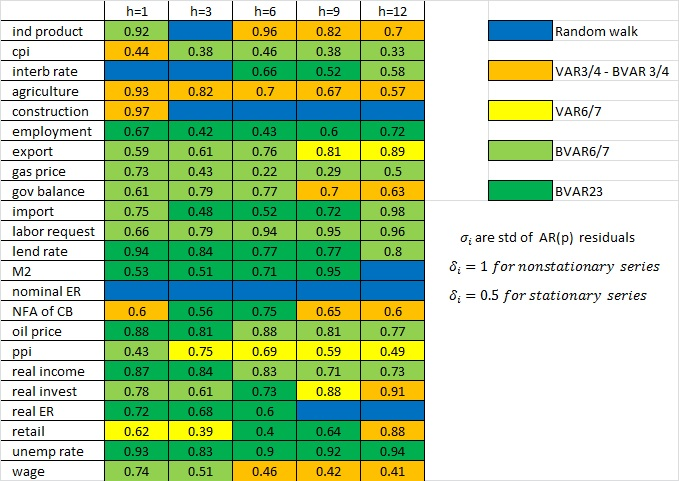
\includegraphics[scale=0.60]{hyper3.jpg}
\end{center}
\end{frame}

\begin{frame}{Robustness check}
\begin{adjustwidth}{-1.5em}{-1.5em}
\vspace{-5mm}
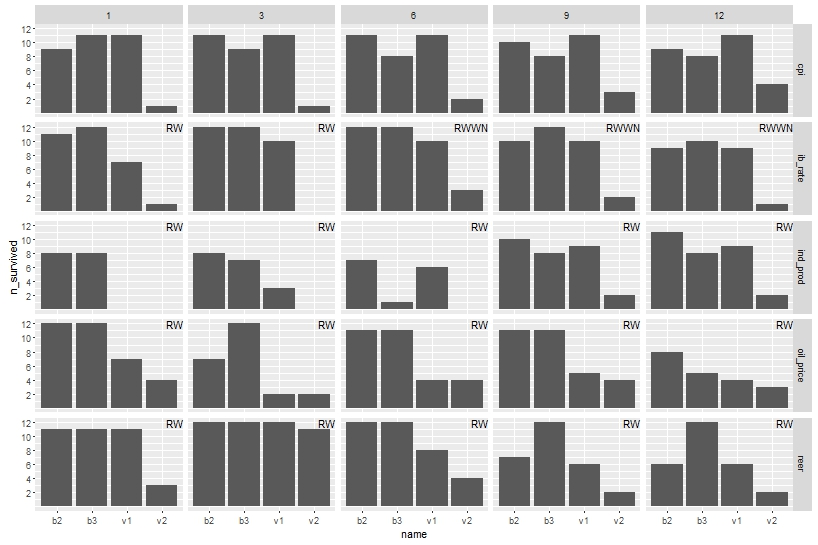
\includegraphics[scale=0.42]{model_selection.jpeg}
\end{adjustwidth}
\end{frame}

\begin{frame}
\frametitle{BVAR vs ARIMA}

\end{frame}


\begin{frame}
\frametitle{BVAR vs ETS}

\end{frame}

\begin{frame}
\frametitle{BVAR vs VAR-LASSO}

\end{frame}

%VAR-LASSO:
%* compared to BVARS: better stability of estimation
%* shorter estimation time: cross-validation of one/two parameters is feasible
%* greater out of sample error
%* too many possible penalty structures
%
%
%
%conclusion:
%best model depends on time series forecasted
%sometimes (but not always!) information from other series is useful
%great demand unique bayesian framework for time series prediction with trend, seasonality and exogenous regressors




\begin{frame}%22
\begin{center}
THANK YOU!
\vspace{1cm}
\end{center}
Boris Demeshev: boris.demeshev@gmail.com\\
Oxana Malakhovskaya: omalakhovskaya@hse.ru\\
Link to the repository: https://github.com/bdemeshev/bvar\_om
\end{frame}
\end{document}
